\documentclass{article}
\usepackage{graphicx}
\usepackage[usenames, dvipsnames]{color}
\definecolor{rosewood}{rgb}{0.4, 0.0, 0.04}
\begin{document}
\begin{center}
\Huge{{\bf\color{rosewood}DEVICE MODELLING LABORATORY}}\\
\vspace{30 mm}
\huge{{\bf\color{rosewood} NGSPICE CODES}}\\
\huge{{\bf\color{rosewood} AND }}\\
\huge{{\bf \color{rosewood}SIMULATIONS}}\\
\end{center}
\vspace{60mm}
\begin{flushright}
\LARGE{{\bf\color{rosewood}SUBMITTED BY :-}}\\
\LARGE{{\bf\color{rosewood} VATSALA  SWAROOP}}\\
\LARGE{{\bf\color{rosewood} BT12ECE086}}\\
\LARGE{{\bf\color{rosewood} N4 BATCH}}\\      
\end{flushright}    
\newpage  


\begin{center}
\Large{{\bf\color{rosewood}ASSIGNMENT NO. 1}}\\*
\vspace{2mm}
\large{{\bf\textcolor{rosewood}{ Simple RC circuit}}}\\*
\vspace{5mm}
\end{center}
\begin{flushleft}
\large{{\bf\textcolor{rosewood}{AIM :-} To study characteristics of RC circuit}}\vspace{5mm}\\*

\large{{\bf\textcolor{rosewood}{THEORY} :-An RC circuit is simply a circuit with a voltage source (battery) connected in series with a resistor and a capacitor.As with circuits made up simply of resistors, electrical currents can flow in this RC circuit, with one 
modification. A battery connected in series with a resistor will produce a constant current. The same battery in series with a capacitor will produce a time varying current, which decays gradually to zero. If the battery is removed and the circuit reconnected without the battery, a current will flow (for a short time) in the opposite direction as the capacitor "discharges". A measure of how long these transient currents last in a given circuit is given by the "time constant", t.
The time it takes for these transient currents to decay depends on the resistance and capacitance.  A first order RC circuit is composed of one resistor and one capacitor and is the simplest type of RC circuit.RC circuits can be used to filter a signal by blocking certain frequencies and passing others. The two most common RC filters are the high-pass filters and low-pass filters; band-pass filters and band-stop filters usually require RLC filters, though crude ones can be made with RC filters.}}\vspace{5mm}\\*

\large{{\bf\textcolor{rosewood}{ CODE} :-
*RC CKT:lab ex1\newline
R1 1 2 1.5k\newline
C1 2 0 0.003n\newline
VIN 1 0 PULSE (0 1.8 0n 2n 2n 50n 100n)\newline
.TRAN 1n 200n\newline
.CONTROL\newline
run\newline
display\newline
plot V(1) V(2)\newline
.endc \newline
.end \newline}}\\*


\begin{figure}[ht] 
\large{{\bf\textcolor{rosewood}{ WAVEFORM} :-}}\vspace{5mm} \\*
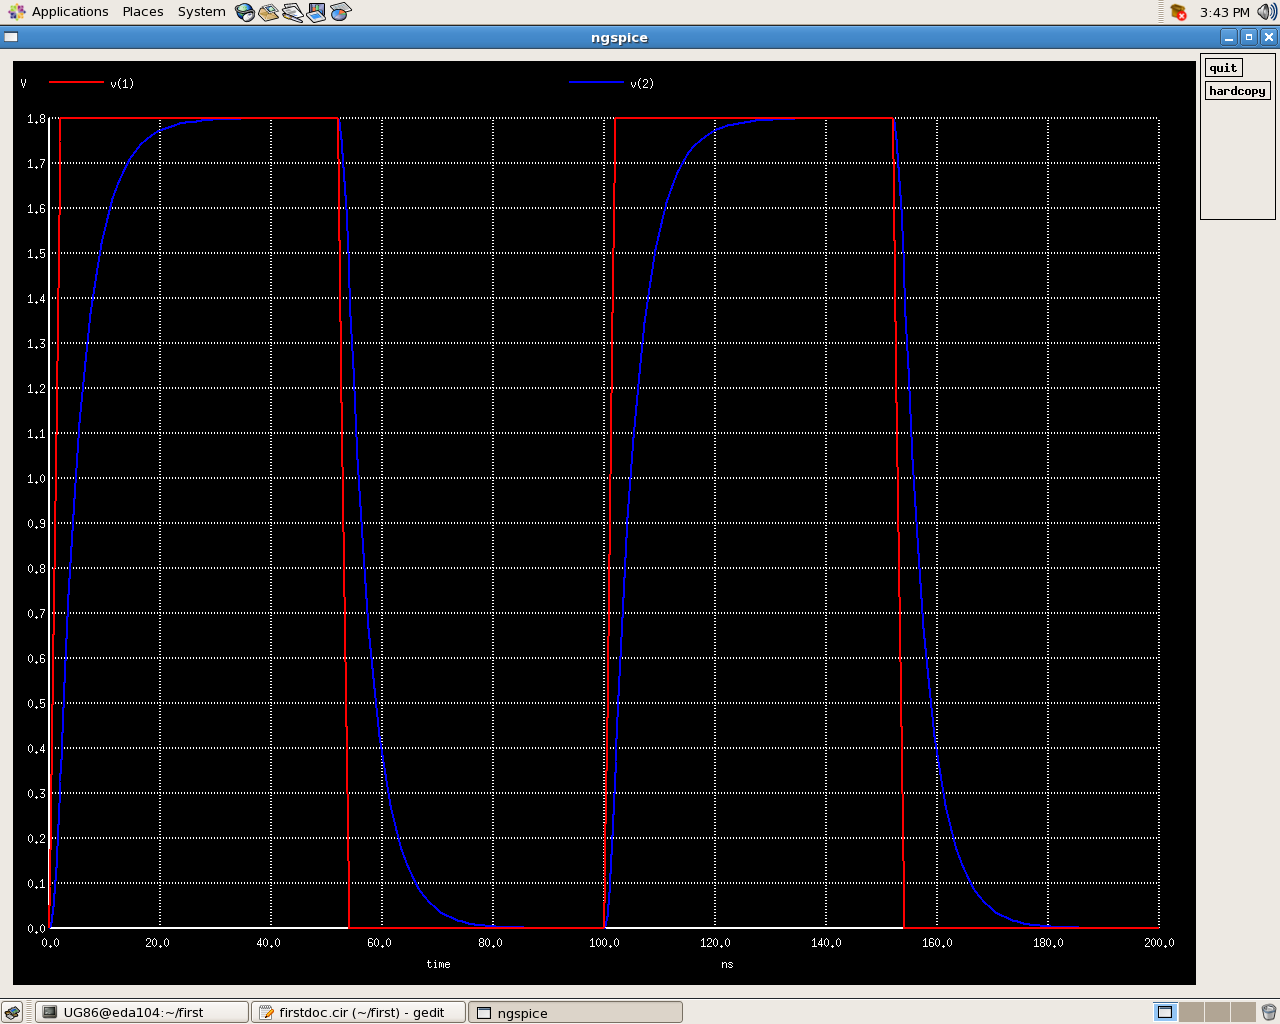
\includegraphics[width=10cm, height=10cm]{rc_first.png} 
\caption{RC circuit waveform}
\label{fig:circuit1} 
\end{figure} 
\end{flushleft}
\newpage




\begin{center}
\Large{{\bf\color{rosewood}ASSIGNMENT NO. 2}}\\*
\vspace{2mm}
\large{{\bf\textcolor{rosewood}{ Diode Characteristics}}}\\*
\vspace{5mm}
\end{center}
\begin{flushleft}
\large{{\bf\textcolor{rosewood}{AIM :-} To study characteristics of Diode}}\vspace{5mm}\\*

\large{{\bf\textcolor{rosewood}{THEORY} :-Semiconductor diode theory is at the very centre of much of today's electronics industry.
One of the fundamental structures within semiconductor technology is the PN junction. The semiconductor diode has the valuable property that electrons only flow in one direction across it and as a result it acts as a rectifier. As it has two electrodes it receives its name - diode. 
A diode characteristic is simply a graph of the voltage applied to a diode and the current it produces. The negative part of the voltage axis corresponds to when the diode is reverse biased and the positive part is when the diode is forward biased. The negative part of the current axis shows current flowing in the reverse direction through the diode.  }}\vspace{5mm}\\*

\large{{\bf\textcolor{rosewood}{ CODE} :-
*Diode ckt:lab ex2\newline
D1 2 3\newline
R1 3 0 10k\newline
vx 1 2 0\newline
VIN 1 0 1 sin(0 1 3k)\newline
.DC VIN 0 5 0.1\newline
.CONTROL\newline
run\newline
display\newline
plot v(1) v(2)\newline
plot vxbranch\newline
.endc\newline
.end\newline}}\\*


\begin{figure}[ht] 
\large{{\bf\textcolor{rosewood}{ WAVEFORM} :-}}\vspace{5mm} \\*
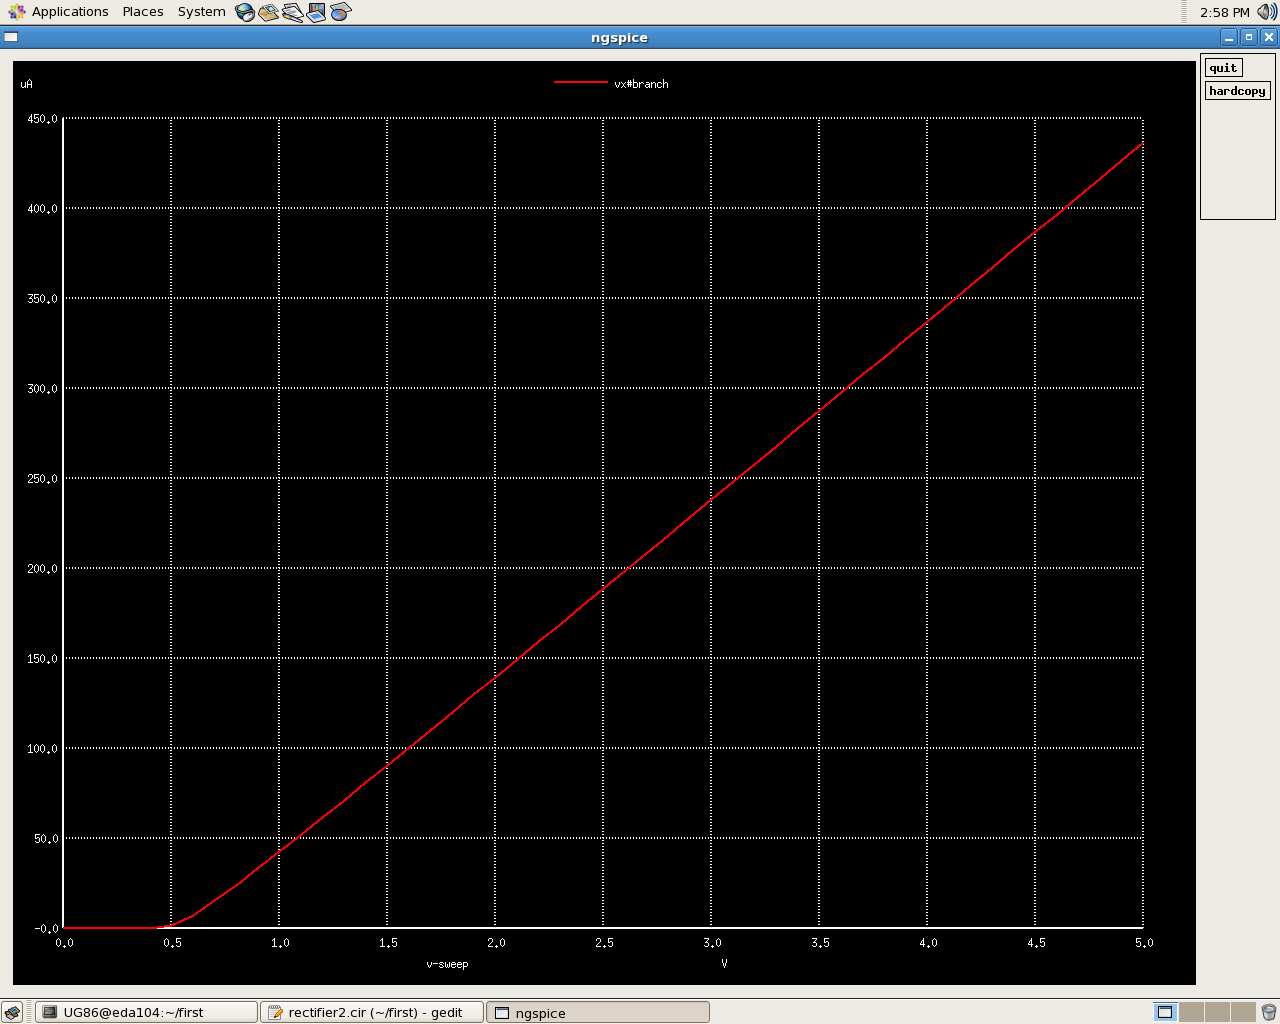
\includegraphics[width=10cm, height=10cm]{diode.png} 
\caption{VI characteristics of diode}
\label{fig:circuit2} 
\end{figure} 
\end{flushleft}
\newpage




\begin{center}
\Large{{\bf\textcolor{rosewood}{ASSIGNMENT NO. 3}}}\\*
\vspace{2mm}
\large{{\bf\textcolor{rosewood}{ Half Wave Rectifier}}}\\*
\vspace{5mm}
\end{center}
\begin{flushleft}
\large{{\bf\textcolor{rosewood}{AIM :-} To study characteristics of  half wave rectifier}}\vspace{5mm}\\*

\large{{\bf\textcolor{rosewood}{THEORY} :-
 The purpose of the rectifier section is to convert the incoming ac from a transformer or other ac power source to some form of pulsating dc. That is, it takes current that flows alternately in both directions , and modifies it so that the output current flows only in one direction.The simplest rectifier circuit is nothing more than a diode connected in series with the ac input, as shown to the right. Since a diode passes current in only one direction, only half of the incoming ac wave will reach the rectifier output. Thus, this is a basic half-wave rectifier.The orientation of the diode matters; as shown, it passes only the positive half-cycle of the ac input, so the output voltage contains a positive dc component. If the diode were to be reversed, the negative half-cycle would be passed insteadRectifiers have many uses, but are often found serving as components of DC power supplies and high-voltage direct current power transmission systems.}}\vspace{5mm}\\*

\large{{\bf\textcolor{rosewood}{ CODE} :-
*RECTIFIER CKT:lab ex3\newline
D1 1 2\newline 
R1 2 0 10k\newline
VIN 1 0 sin(0 2 1k)\newline
.TRAN 1n 2m\newline
.CONTROL\newline
run\newline
display\newline
plot V(1) V(2)\newline
.endc\newline
.end\newline}}\\*

\begin{figure}[ht] 
\large{{\bf\textcolor{rosewood}{ WAVEFORM} :-}}\vspace{5mm} \\*
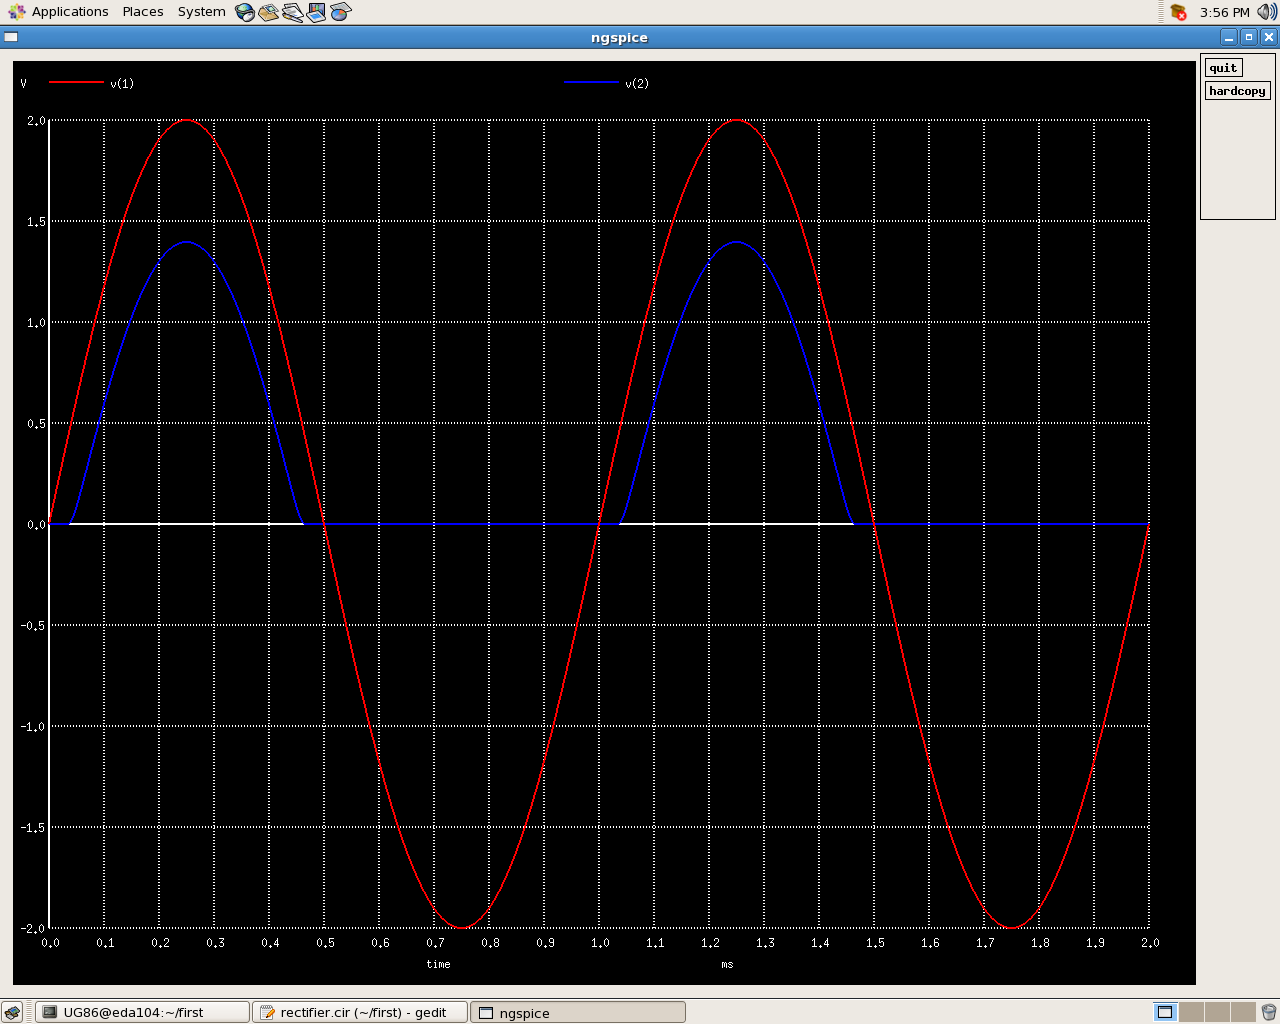
\includegraphics[width=10cm, height=10cm]{rectifier.png} 
\caption{rectifier circuit output} 
\label{fig:circuit2} 
\end{figure} 
\end{flushleft}
\newpage 




\begin{center}
\Large{{\bf\color{rosewood}ASSIGNMENT NO. 4}}\\*
\vspace{2mm}
\large{{\bf\textcolor{rosewood}{ Filter}}}\\*
\vspace{5mm}
\end{center}
\begin{flushleft}
\large{{\bf\textcolor{rosewood}{AIM :-} To study characteristics of filter circuit}}\vspace{5mm}\\*

\large{{\bf\textcolor{rosewood}{THEORY} :-An RC circuit is simply a circuit with a voltage source (battery) connected in series with a resistor and a capacitor.As with circuits made up simply of resistors, electrical currents can flow in this RC circuit, with one 
modification. A battery connected in series with a resistor will produce a constant current. The same battery in series with a capacitor will produce a time varying current, which decays gradually to zero. If the battery is removed and the circuit reconnected without the battery, a current will flow (for a short time) in the opposite direction as the capacitor "discharges". A measure of how long these transient currents last in a given circuit is given by the "time constant", t.
The time it takes for these transient currents to decay depends on the resistance and capacitance.  A first order RC circuit is composed of one resistor and one capacitor and is the simplest type of RC circuit.RC circuits can be used to filter a signal by blocking certain frequencies and passing others. The two most common RC filters are the high-pass filters and low-pass filters; band-pass filters and band-stop filters usually require RLC filters, though crude ones can be made with RC filters.}}\vspace{5mm}\\*

\large{{\bf\textcolor{rosewood}{ CODE} :-
*capacitor RECTIFIER CKT:lab ex4\newline
D1 1 2 \newline
R1 2 0 10k\newline
C1 2 0 0.1u\newline
VIN 1 0 sin(0 2 1k)\newline
.TRAN 1n 2m\newline
.CONTROL\newline
run\newline
display\newline
plot V(1) V(2)\newline
.endc\newline
.end\newline}}\\*


\begin{figure}[ht] 
\large{{\bf\textcolor{rosewood}{ WAVEFORM} :-}}\vspace{5mm} \\*
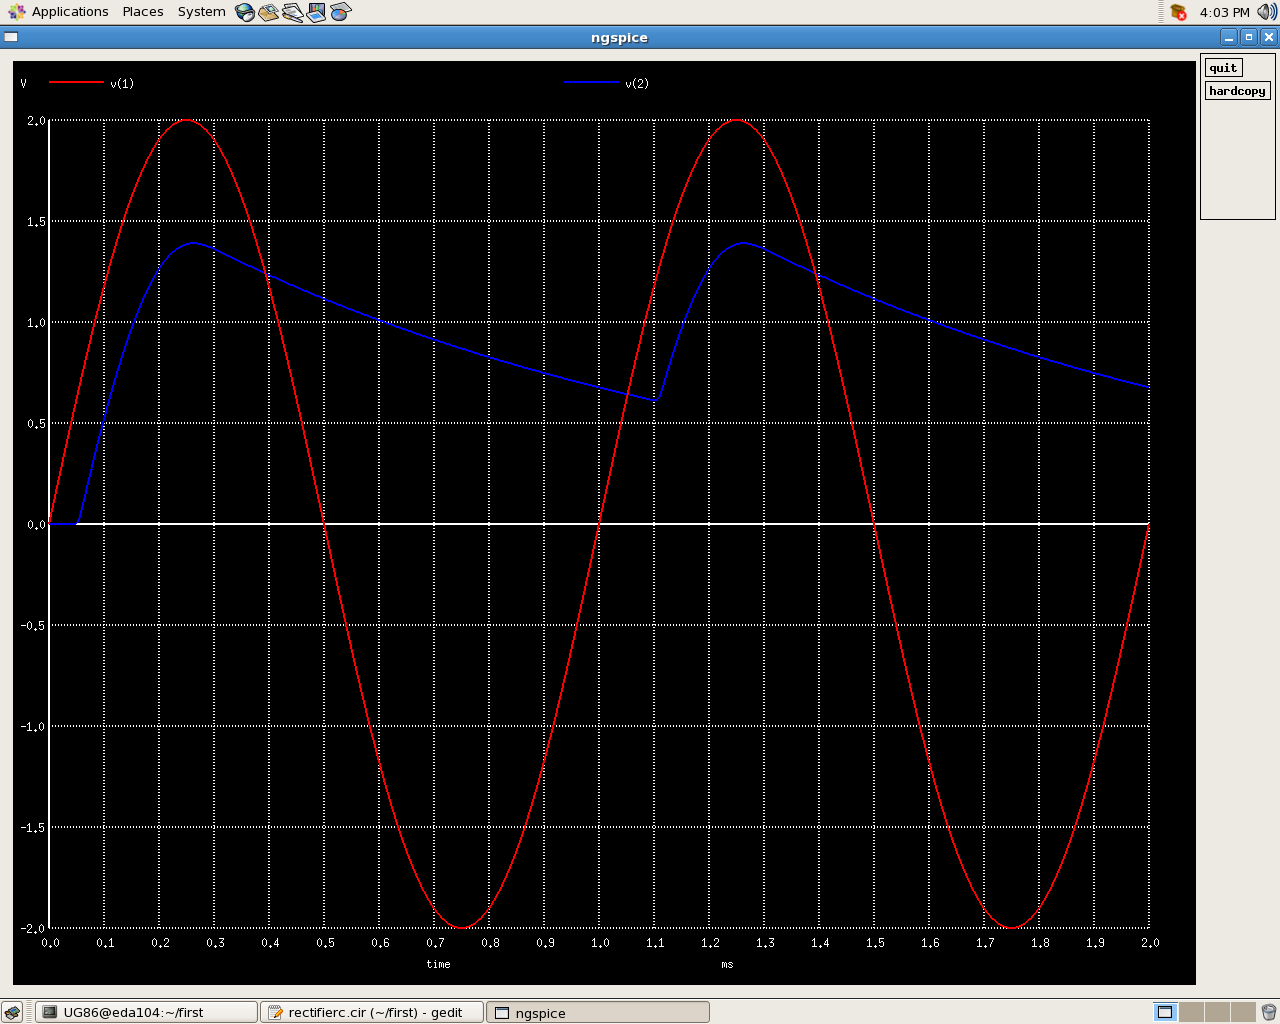
\includegraphics[width=10cm, height=10cm]{filter.png} 
\caption{Filter circuit waveform}
\label{fig:circuit4} 
\end{figure} 
\end{flushleft}
\newpage




\begin{center}
\Large{{\bf\textcolor{rosewood}{ASSIGNMENT NO. 5}}}\\*
\vspace{2mm}
\large{{\bf \textcolor{rosewood}{Common Emitter Amplifier}}}\\*
\vspace{5mm}
\end{center}
\begin{flushleft}
\large{{\bf\textcolor{rosewood}{AIM :-} To study characteristics of Common Emitter Amplifier}}\vspace{5mm}\\*

\large{{\bf\textcolor{rosewood}{THEORY :-}
In electronics, a common emitter amplifier is one of three basic single-stage bipolar-junction-transistor (BJT) amplifier topologies, typically used as a voltage amplifier.The common emitter transistor amplifier is possibly the most widely used transistor configuration.The common emitter transistor amplifier circuit is often seen as the standard format for a transistor circuit where voltage gain is required.It is often used in small class A linear amplifier stages as well as logic outputs and many other areas. Here, its characteristics lend themselves to this form of application.}}\vspace{5mm}\\*
\large{{\bf\textcolor{rosewood}{CODE :-}
*Common Emitter Amplifier \newline
Vcc 3 0 DC 12 \newline
Cin 1 2 1u \newline
R1 3 2 25k \newline
R2 2 0 5k \newline
R3 3 4 1.5k \newline
R4 5 0 220 \newline
Q1 4 2 5 Qn \newline
Ce 5 0 10u \newline
Co 4 6 10o \newline
R5 6 0 2k \newline
\newline
.model Qn npn CJE=50pf CJS=50pf CJC=50pf \newline
\newline
Vin 1 0 SIN(0 10m 1k) \newline
.tran 1u 2m \newline
.control \newline
run \newline
display \newline
plot V(1)  V(6) \newline
.endc \newline
.end \newline}}\\*
\begin{figure}[ht]
\large{{\bf\textcolor{rosewood}{ WAVEFORM} :-}}\vspace{5mm} \\*
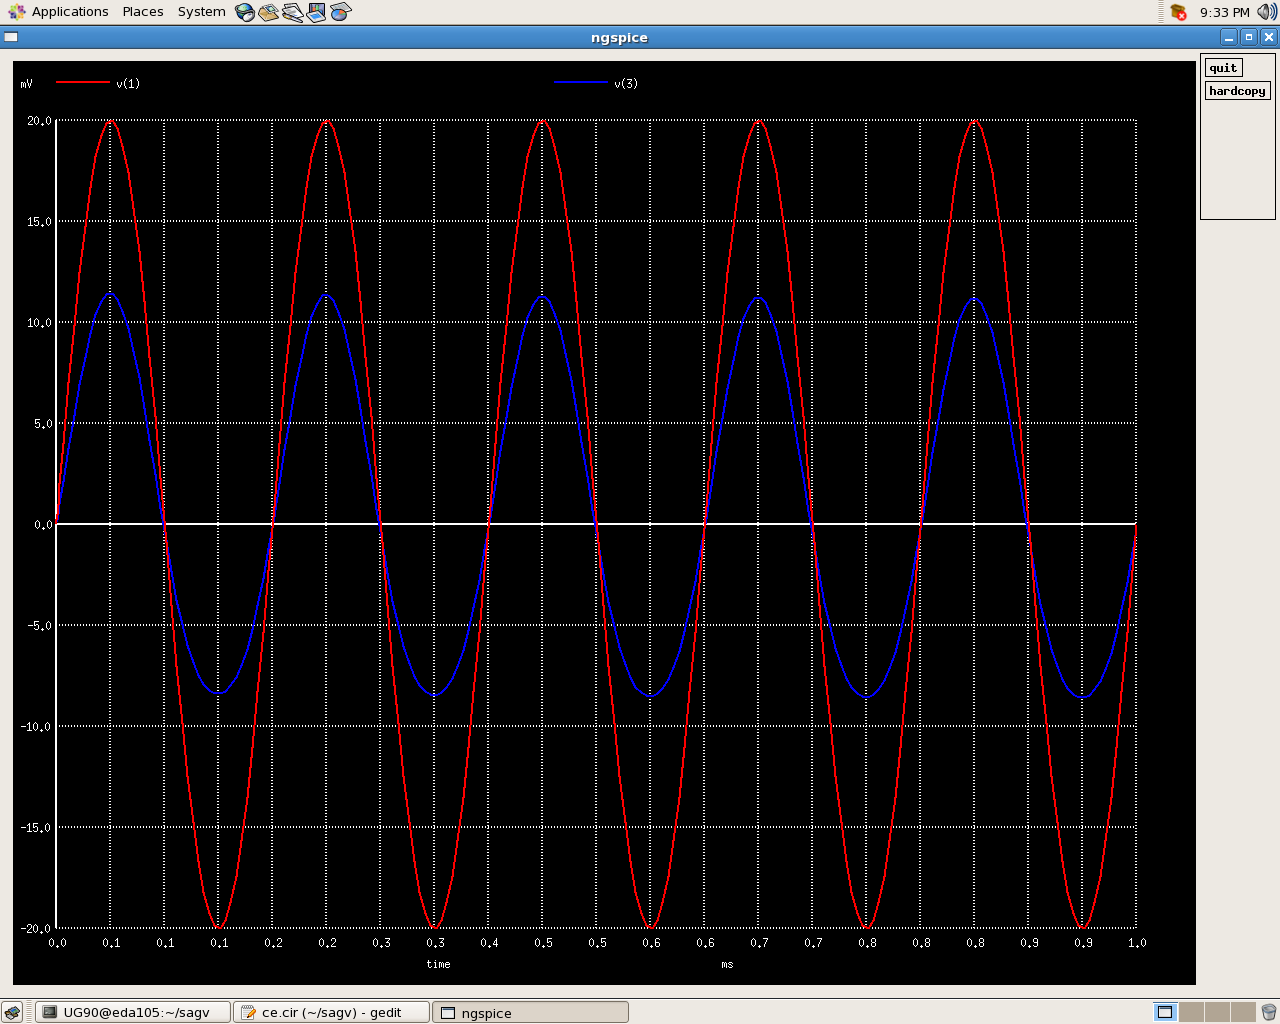
\includegraphics[width=10cm, height=10cm]{ce.png}
\caption{ceamp output} 
\label{fig:circuit3} 
\end{figure}
\end{flushleft}
\newpage




\begin{center}
\Large{{\bf\textcolor{rosewood}{ASSIGNMENT NO. 6}}}\\*
\vspace{2mm}
\large{{\bf\textcolor{rosewood}{ Common Emitter Amplifier AC analysis}}}\\*
\vspace{5mm}
\end{center}
\begin{flushleft}
\large{{\bf\textcolor{rosewood}{AIM :-}To study ac analysis of ce amplifier}}\vspace{5mm}\\*
\large{{\bf\textcolor{rosewood}{THEORY :-}
In electronics, a common emitter amplifier is one of three basic single-stage bipolar-junction-transistor (BJT) amplifier topologies, typically used as a voltage amplifier.The common emitter transistor amplifier is possibly the most widely used transistor configuration.The common emitter transistor amplifier circuit is often seen as the standard format for a transistor circuit where voltage gain is required.It is often used in small class A linear amplifier stages as well as logic outputs and many other areas. Here, its characteristics lend themselves to this form of application.}}\vspace{5mm}\\*
\large{{\bf\textcolor{rosewood}{CODE :-}
*Common Emitter Amplifier \newline
Vcc 3 0 DC 12 \newline
Cin 1 2 1u \newline
R1 3 2 25k \newline
R2 2 0 5k \newline
R3 3 4 1.5k \newline
R4 5 0 220 \newline
Q1 4 2 5 Qn \newline
Ce 5 0 10u \newline
Co 4 6 10o \newline
R5 6 0 2k \newline
\newline
.model Qn npn CJE=50pf CJS=50pf CJC=50pf \newline
\newline
Vin 1 0 AC 10m \newline
.ac DEC 100 100 1000MEG \newline
.control \newline
run \newline
display \newline
plot abs(V(6)) \newline
.endc \newline
.end \newline
}}\\*
\begin{figure}[ht] 
\large{{\bf\textcolor{rosewood}{ WAVEFORM} :-}}\vspace{5mm} \\*
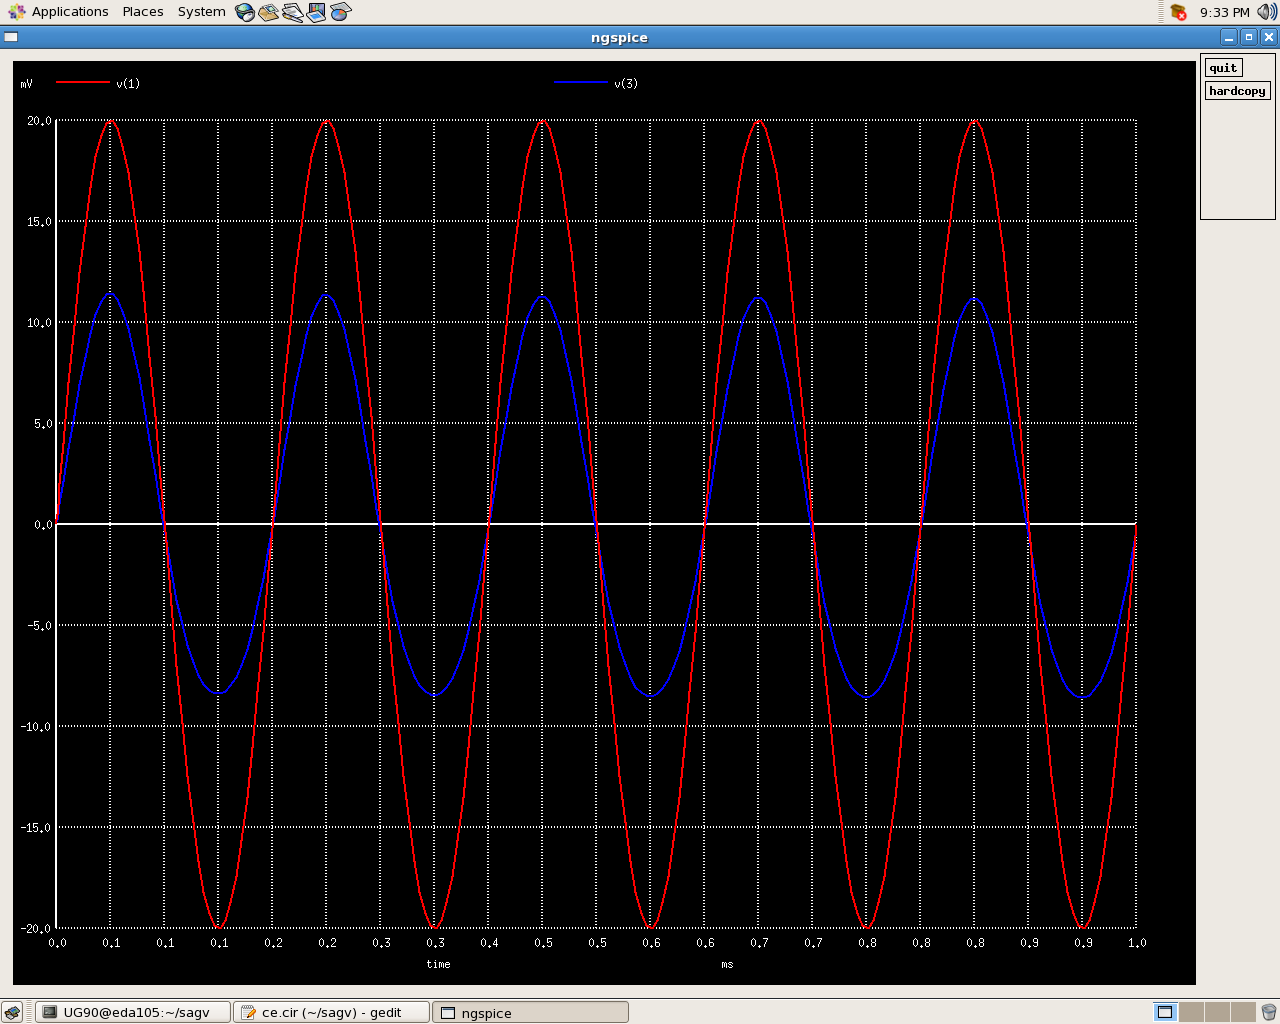
\includegraphics[width=10cm, height=10cm]{ce.png}
\caption{ceamp output ac analysis} 
\label{fig:circuit4} 
\end{figure}

\end{flushleft}
\end{document}